% !TeX root = er.tex

\chapter{Sensors}\label{ch.sensors}
\index{sensor}

\abstract*{Robots must sense their environment. Sensors use ultrasound, infrared and lasers to determine distance and angles. Cameras are essential for identifying objects in the environment. Important properties of sensors are their range, resolution, precision and accuracy. The response of a sensor may be linear, but if not calibration is performed so that values returned by the sensor can be interpreted as physical quantities.}

A robot cannot move a specific distance in a specific direction just by setting the relative power of the motors of the two wheels and the period of time that the motors run. Suppose that we want the robot to move straight ahead. If we set the power of the two motors to the same level, even small differences in the characteristics of the motors and wheels will cause the robot turn slightly to one side. Unevenness in the surface over which the robot moves will also cause the wheels to turn at different speeds. Increased or decreased friction between the wheels and the surface can affect the distance moved in a specific period of time. Therefore, if we want  robot to move towards a wall 1 m away and stop 20 cm in front of it, the robot must \emph{sense} the existence of the wall and stop when it \emph{detects} that the wall is 20 cm away.

A \emph{sensor} is a component that measures some aspects of the environment. The computer in the robot uses these measurements to control the actions of the robot. One of the most important sensors in robotics is the distance sensor that measures the distance from the robot to an object. By using multiple distance sensors or by rotating the sensor, the angle of the object relative to the front of the robot can be measured. Inexpensive distance sensors using infrared light or ultrasound are invariably used in educational robots; industrial robots frequently use expensive laser sensors because they are highly accurate.

Sound and light are also used for \emph{communications} between two robots as described in Chap.~\ref{ch.swarm}.

More extensive knowledge of the environment can be obtained by analyzing images taken by a camera. While cameras are very small and inexpensive (every smartphone has one), the amount of data in an image is very large and image-processing algorithms require significant computing resources. Therefore, cameras are primarily used in complex applications like self-driving cars.

Section~\ref{s.classify} introduces the terminology of sensors. Section~\ref{s.distance-sensors} presents distance sensors, the sensors most often used by educational robots. This is followed by Sect.~\ref{s.cameras} on cameras and then a short section on other sensors that robots use (Sect.~\ref{s.other-sensors}). Section~\ref{s.range} defines the characteristics of sensors: range, resolution, precision, accuracy. The chapter concludes with a discussion of the nonlinearity of sensors (Sect.~\ref{s.nonlinearity}).

\section{Classification of sensors}\label{s.classify}

Sensors are classified as \emph{proprioceptive}\index{sensor!proprioceptive} or \emph{exteroceptive}\index{sensor!exteroceptive}, and exteroceptive sensors are further classified as \emph{active} or \emph{passive} (Fig.~\ref{fig.sensor-classification}). A proprioceptive sensor measures something internal to the robot itself. The most familiar example is a car's speedometer which measures the car's speed by counting rotations of the wheels (Sect.~\ref{s.wheel}). An exteroceptive sensor measures something external to the robot such as the distance to an object. An active sensor affects the environment usually by emitting energy: a sonar range finder on a submarine emits sound waves and uses the reflected sound to determine range. A passive sensor does not affect the environment: a camera simply records the light reflected off an object. Robots invariably use some exteroceptive sensors to correct for errors that might arise from proprioceptive sensors or to take changes of the environment into account.

\begin{figure}
\begin{center}
\begin{tikzpicture}[node distance = 4mm and 1cm]
\node (sensor) { \textsf{sensor} };
\node (ex) [above right=of sensor] { \textsf{exteroceptive} };
\node (pro) [below right=of sensor] { \textsf{proprioceptive} };
\node (active) [above right=of ex] { \textsf{active} };
\node (passive) [below right=of ex] { \textsf{passive} };
\draw (sensor) -- (pro);
\draw (sensor) -- (ex);
\draw (ex) -- (active);
\draw (ex) -- (passive);
\end{tikzpicture}
\caption{Classification of sensors}\label{fig.sensor-classification}
\end{center}
\end{figure}

\section{Distance sensors}\label{s.distance-sensors}
\index{sensor!distance}

In most applications, the robot needs to measure the distance from the robot to an object using a \textit{distance sensor}. Distance sensors are usually \emph{active}: they transmit a signal and then receive its reflection (if any) from an object (Fig.~\ref{fig.measure-d}). One way of determining distance is to measure the time that elapses between sending a signal and receiving it:
\begin{equation}
s = \frac{1}{2}vt\,,\label{eq.reflected}
\end{equation}
where $s$ is the distance, $v$ is the velocity of the signal and $t$ is the elapsed time between sending and receiving the signal. The factor of one-half takes into account that the signal travels the distance twice: to the object and then reflected back. Another way of reconstructing the distance is by using triangulation as explained in Sect.~\ref{s.triangulating-sensors}.

\begin{figure}
\begin{center}
\begin{tikzpicture}
\draw[xshift=-1mm] pic { robot };
\foreach \x in {14, 18, 22, 26, 30, 34}
\draw[blue] (\x mm,-10mm) arc[start angle=-30, end angle=30, radius=20mm];
\draw[fill] (38mm,0) circle[radius=3pt];
\foreach \x in {16, 20, 24, 28, 32, 36}
\draw[thick,dashed,red] (\x mm,-10mm) arc[start angle=210, end angle=150, radius=20mm];
\end{tikzpicture}
\end{center}
\caption{Measuring distance by transmitting a wave and receiving its reflection}\label{fig.measure-d}
\end{figure}

Low-cost distance sensors are based on another principle: since the intensity of a signal decreases with distance, measuring the intensity of a reflected signal gives an indication of the distance from the sensor to an object. The disadvantage of this method is that the intensity of the received signal is influenced by factors such as the reflectivity of the object.


\subsection{Ultrasound distance sensors}
\index{sensor!ultrasound}

Ultrasound is sound whose frequency is above $20,000$ hertz, higher than the highest frequency that can be heard by the human ear. There are two environments where sound is better than vision: at night and in water. Bats use ultrasound for navigating when flying at night because after the sun sets there is little natural light for locating food. Ships and submarines use ultrasound for detecting objects because sound travels much better in water than it does in air. Check this yourself by going for a swim in a muddy lake or in the ocean: How far away can you see a friend? Now, ask him to make a sound by hitting two objects together or by clapping his hands. How far away can you hear the sound? 

The speed of sound in air is about $340$ m/s or $34,000$ cm/s. If an object is at a distance of $34$ cm from a robot, from Eq.~\ref{eq.reflected} it follows that an ultrasound signal will travel to the object and be reflected back in:
\[\frac{2\cdot 34}{34000} = \frac{2}{1000} = 2\times 10^{-3}\  \textrm{seconds} = 2\  \textrm{milliseconds}.\]
An electronic circuit can easily measure periods of time in milliseconds.

The advantage of ultrasound sensors is that they are not sensitive to changes in the color or light reflectivity of objects, nor to the light intensity in the environment. They are, however, sensitive to texture: fabric will absorb some of the sound, while wood or metal will reflect almost all the sound. That is why curtains, carpets and soft ceiling tiles are used to make rooms more comfortable.

Ultrasound sensors are relatively cheap and can work in outdoor environments. They are used in cars for detecting short distances, such as to aid in parking. Their main disadvantage is that the distance measurement is relatively slow, since the speed of sound is much less than the speed of light. Another disadvantage is that they cannot be focused in order to measure the distance to a specific object.

\subsection{Infrared proximity sensors}
\index{sensor!infrared}\index{sensor!proximity}

\emph{Infrared light} is light whose wavelength is longer than red light, which is the light with the longest wavelength that our eyes can see. The eye can see light with wavelengths from about $390$ to $700$ nanometers (a nanometer is one-millionth of a millimeter). Infrared light has wavelengths between $700$ and $1000$ nanometers. It is invisible to the human eye and is therefore used in the remote control of TV sets and other electronic appliances.

Proximity sensors are simple devices that use light to detect the presence of an object by measuring the intensity of the reflected light. Light intensity decreases with the square of the distance from the source and this relationship can be used to measure the approximate distance to the object. The measurement of the distance is not very accurate because the reflected intensity also depends on the reflectivity of the object. A black object reflects less light than a white object placed at the same distance, so a proximity sensor cannot distinguish between a close black object and a white object placed somewhat farther away. This is the reason why these sensors are called \emph{proximity} sensors, not distance sensors. Most educational robots use proximity sensors because they are much less expensive than distance sensors.

\subsection{Optical distance sensors}\label{s.optical-distance}
\index{sensor!optical}

Distance can be computed from a measurement of the elapsed time between sending a light signal and receiving it. The light can be ordinary light or light from a laser. Light produced by a laser is \emph{coherent} (see below).  Most commonly, lasers for measuring distance use infrared light, although visible light can also be used. Lasers have several advantages over other light sources. First, lasers are more powerful and can detect and measure the distance to objects at long range. Second, a laser beam is highly focused, so an accurate measurement of the angle to the object can be made (Fig.~\ref{fig.beam}).

\begin{figure}
\begin{center}
\begin{tikzpicture}
\draw pic { robot };
\draw[fill] (20:5) circle[radius=3pt];
\draw[blue] (0,0) -- (17:5) arc[start angle=17, end angle=23, radius=5cm] -- cycle;
\draw[dashed,red] (0,0) -- (10:5) arc[start angle=10, end angle=30, radius=5cm] -- cycle;
\end{tikzpicture}
\end{center}
\caption{Beam width of laser light (solid) and non-coherent light (dashed)}\label{fig.beam}
\end{figure}

\begin{quote}
\begin{center}
\textbf{Coherent light}
\end{center}
Three types of light are shown in Fig.~\ref{fig.coherent}. The light from the sun or a light bulb is called \emph{white light} because it is composed of light of many different colors (frequencies), emitted at different times (phases) and emitted in different directions. Light-emitting diodes (LED) emit \emph{monochromatic light} (light of a single color), but they are non-coherent because their phases are different and they are emitted in different directions. Lasers emit \emph{coherent light}: all waves are of the same frequency and the same phase (the start of each wave is at the same time). All the energy of a light is concentrated in a narrow beam and distance can be computed by measuring the time of flight and the difference in phase of the reflected light.
\end{quote}

\begin{figure}
\begin{center}
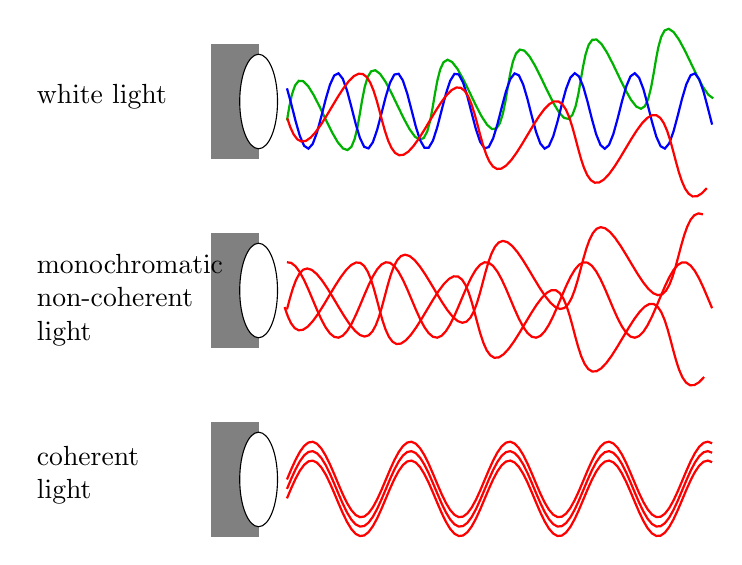
\begin{tikzpicture}[scale=.6,domain=0:9,align=left]
\draw[fill,gray] (-16mm,-8mm) rectangle +(10mm,24mm);
\draw[fill=white] (-6mm,4mm) circle[x radius=4mm, y radius=10mm];
\node[anchor=west] at (-5.5,5mm) {\p{white light}};
\draw[samples=100,green!70!black,thick,rotate=8] plot (\x,{.8*sin(4*\x r)});
\draw[samples=100,blue,thick,yshift=2mm] plot (\x,{.8*sin(5*(\x+.5) r)});
\draw[samples=100,red,thick,rotate=-8,yshift=4mm] plot (\x,{.8*sin(3*(\x+1.2) r)});
\begin{scope}[yshift=-4cm]
\draw[fill,gray] (-16mm,-8mm) rectangle +(10mm,24mm);
\draw[fill=white] (-6mm,4mm) circle[x radius=4mm, y radius=10mm];
\node[anchor=west] at (-5.5,2mm) {\p{monochromatic}\\\p{non-coherent}\\\p{light}};
\draw[samples=100,red,thick,rotate=8] plot (\x,{.8*sin(3*\x r)});
\draw[samples=100,red,thick,yshift=2mm] plot (\x,{.8*sin(3*(\x+.5) r)});
\draw[samples=100,red,thick,yshift=4mm,rotate=-8] plot (\x,{.8*sin(3*(\x+1.2) r)});
\end{scope}
\begin{scope}[yshift=-8cm]
\draw[fill,gray] (-16mm,-8mm) rectangle +(10mm,24mm);
\draw[fill=white] (-6mm,4mm) circle[x radius=4mm, y radius=10mm];
\node[anchor=west] at (-5.5,5mm) {\p{coherent}\\\p{light}};
\draw[samples=100,red,thick] plot (\x,{.8*sin(3*\x r)});
\draw[samples=100,red,thick,yshift=2mm] plot (\x,{.8*sin(3*\x r)});
\draw[samples=100,red,thick,yshift=4mm] plot (\x,{.8*sin(3*\x r)});
\end{scope}
\end{tikzpicture}
\end{center}
\caption{White, monochromatic and coherent light}\label{fig.coherent}
\end{figure}

Suppose that a pulse of light is transmitted by the robot, reflected off an object and received by a sensor on the robot. The speed of light in air is about $300,000,000$ m/s, which is $3\times 10^8$ m/s or $3\times 10^{10}$ cm/s in scientific notation. If a light signal is directed at an object $30$ cm from the robot, the time for the signal to be transmitted and received is (Fig.~\ref{fig.ir}):\index{sensor!elapsed time}
\[\frac{2\cdot 30}{3\times 10^{10}} = \frac{2}{10^9} = 2\times 10^{-9}\  \textrm{seconds} = 0.002\  \textrm{microseconds}.\]
This is a very short period of time but it can be measured by electronic circuits.

\begin{figure}
\sidecaption
\includegraphics[width=.6\textwidth]{time-of-flight}
\caption{A time of flight distance sensor (black) mounted on a 1.6 mm thick printed circuit (green).}\label{fig.ir}
\end{figure}

The second principle of distance measurement by a light beam is triangulation. In this case the transmitter and the receiver are placed at different locations. The receiver detects the reflected beam at a position that is function of the distance of the object from the sensor.

\subsection{Triangulating sensors}\label{s.triangulating-sensors}

Before explaining how a \emph{triangulating sensor}\index{sensor!triangulating} works, we have to understand how the reflection of light depends on the object it hits. When a narrow beam of light like the coherent light from a laser hits a shiny surface like a mirror, the light rays bounce off in a narrow beam. The angle of reflection relative to the surface of the object is the same as the angle of incidence. This is called \emph{specular} reflection (Fig.~\ref{fig.reflect-left}). When the surface is rough the reflection is \emph{diffuse} (Fig.~\ref{fig.reflect-right}) in all directions because even very close areas of the surface have slightly different angles. Most objects in an environment like people and walls reflect diffusely, so to detect reflected laser light the detector need not be placed at a precise angle relative to the transmitter.

\begin{figure}
\subfigures
\begin{minipage}{\textwidth}
\leftfigure[c]{
\begin{tikzpicture}
\draw(5,0) arc[start angle=270, end angle=90, radius=8mm];
\begin{scope}[rotate=-15,xshift=-6mm,yshift=10mm]
\node[draw,rectangle,anchor=west,minimum height=5mm,minimum width=12mm,transform shape] (laser) at (0,8mm) {\p{Laser}};
\node[draw,rectangle,node distance=-.4pt,minimum height=2mm,minimum width=4mm,transform shape] (tip) [right=of laser] {};
\end{scope}
\draw(tip.east) -- ++(-15:28.5mm) -- +(195:30mm);
\end{tikzpicture}
}
\hspace{\fill}
\rightfigure[c]{
\begin{tikzpicture}
\draw(5,0) arc[start angle=270, end angle=90, radius=8mm];
\begin{scope}[rotate=-15,xshift=-6mm,yshift=10mm]
\node[draw,rectangle,anchor=west,minimum height=5mm,minimum width=12mm,transform shape] (laser) at (0,8mm) {\p{Laser}};
\node[draw,rectangle,node distance=-.4pt,minimum height=2mm,minimum width=4mm,transform shape] (tip) [right=of laser] {};
\end{scope}
\draw(tip.east) -- ++(-15:28.5mm) coordinate (reflect) -- +(195:10mm);
\foreach \angle in {120,135,150,180,210,225}
  \draw(reflect) -- +(\angle:10mm);
\end{tikzpicture}
}
\leftcaption{Specular reflection\label{fig.reflect-left}}
\rightcaption{Diffuse reflection\label{fig.reflect-right}}
\end{minipage}
\end{figure}

Figures~\ref{fig.triangulation-left}--\ref{fig.triangulation-right} show a simplified triangulating sensor detecting an object at two distances. The sensor consists of a laser transmitter and at a distance $d$ away a lens that focuses the received light onto an array of sensors placed at a distance $l$ behind the lens. Assuming that the object reflects light diffusely, some of the light will be collected by the lens and focused onto the sensors. The distance $d$ along the sensor array is inversely proportional to the distance $s$ of the object from the laser emitter.

The triangles $\triangle ll'd'$ and $\triangle ss'd$ are similar, so we have the formula:
\[
\frac{s}{d} = \frac{l}{d'}\,.
\]
Since $l$ and $d$ are fixed by construction, by measuring $d'$ from the index of the sensor which detects the focused light, we can compute $s$, the distance of the object from the sensor. The sensor has to be calibrated by measuring the distance $s$ corresponding to each sensor within the array, but once a table is stored within the computer, the distance $s$ can be performed by a table lookup.

There are many design parameters that affect the performance of a triangulating distance sensor: the power of the laser, the optical characteristics of the lens, the number of sensors in the array and their sensitivity. In addition to the usual trade-off of performance and cost, the main trade-off is between the range and the minimal distance at which an object can be measured. For a very short distance $s$, the size of the detector array $d'$ becomes very large and this puts a practical limit on the minimal distance. The minimal distance can be made shorter by increasing the distance between the laser emitter and the detector array, but this reduces the range. A triangulating sensor can be characterized by the distance $s_{\textit{opt}}$ for optimal performance, the minimal distance and the range around $s_{\textit{opt}}$ at which measurements can be made.

\begin{figure}
\subfigures
\begin{minipage}{\textwidth}
\leftfigure[c]{
\begin{tikzpicture}[scale=.9]
\draw(0,0) rectangle +(3,4);
\node[draw,rectangle,anchor=west,minimum height=5mm,minimum width=12mm] (laser) at (10mm,32mm) {\p{Laser}};
\node[draw,rectangle,node distance=-.4pt,minimum height=2mm,minimum width=2.4mm] (tip) [right=of laser] {};
\draw(26mm,20mm) coordinate (lens) ellipse [x radius=2mm, y radius=4mm];
\draw(26mm,14mm) node {\p{Lens}};
\foreach \y in {8mm,10mm,12mm,14mm,16mm,18mm,20mm,22mm}
  \draw(10mm,\y) circle[radius=1mm];
\draw(11mm,4mm) node {\p{Detector array}};
\node[draw,rectangle,fill,color=lightgray,minimum height=8mm,minimum width=2mm] (object) at (70mm,32mm) {};
\draw(66mm,25mm) node {\p{Object}};
% Triangles
\draw[thick,blue] (tip.east) -- node[right,black] {$d$} (lens.center);
\draw[thick,green!60!black,densely dashed] (lens.center) -- node[above,black] {$l$} +(-16mm,0) coordinate (sensor);
\draw[blue,thick] (sensor) -- node[left,black] {$d'$} ($ (object.west) ! 1.373 ! (lens.center) $) coordinate (sensor1);
\draw[densely dashed,thick,green!60!black] (tip.east) -- node[above,black] {$s$} (object.west);
\draw[red,thick] (object.west) -- ($ (object.west) ! 1.373 ! (lens.center) $) coordinate (sensor1);
\fill(tip.east) circle[radius=.8pt];
\fill(lens.center) circle[radius=.8pt];
\fill(sensor) circle[radius=.8pt];
\fill(sensor1) circle[radius=.8pt];
\node at (48mm,24mm) {$s'$};
\node at (18mm,14mm) {$l'$};
\end{tikzpicture}
}
\hspace{\fill}
\rightfigure[c]{
\begin{tikzpicture}[scale=.9]
\draw(0,0) rectangle +(3,4);
\node[draw,rectangle,anchor=west,minimum height=5mm,minimum width=12mm] (laser) at (10mm,32mm) {\p{Laser}};
\node[draw,rectangle,node distance=-.4pt,minimum height=2mm,minimum width=2.4mm] (tip) [right=of laser] {};
\draw(26mm,20mm) coordinate (lens) ellipse [x radius=2mm, y radius=4mm];
\draw(26mm,14mm) node {\p{Lens}};
\foreach \y in {8mm,10mm,12mm,14mm,16mm,18mm,20mm,22mm}
  \draw(10mm,\y) circle[radius=1mm];
\draw(11mm,4mm) node {\p{Detector array}};
\node[draw,rectangle,fill,color=lightgray,minimum height=8mm,minimum width=2mm] (object) at (50mm,32mm) {};
\draw(46.5mm,25mm) node {\p{Object}};
% Triangles
\draw[thick,blue] (tip.east) -- node[right,black] {$d$} (lens.center);
\draw[thick,green!60!black,densely dashed] (lens.center) -- node[above,black] {$l$} +(-16mm,0) coordinate (sensor);
\draw[blue,thick] (sensor) -- node[left,black] {$d'$} ($ (object.west) ! 1.7 ! (lens.center) $) coordinate (sensor1);
\draw[densely dashed,thick,green!60!black] (tip.east) -- node[above,black] {$s$} (object.west);
\draw[red,thick] (object.west) -- ($ (object.west) ! 1.7 ! (lens.center) $) coordinate (sensor1);
\fill(tip.east) circle[radius=.8pt];
\fill(lens.center) circle[radius=.8pt];
\fill(sensor) circle[radius=.8pt];
\fill(sensor1) circle[radius=.8pt];
\node at (38mm,24mm) {$s'$};
\node at (18mm,14mm) {$l'$};
\end{tikzpicture}
}
\leftcaption{Triangulation of a far object\label{fig.triangulation-left}}
\rightcaption{Triangulation of a near object\label{fig.triangulation-right}}
\end{minipage}
\end{figure}

\subsection{Laser scanners}
\index{sensor!laser}

When ultrasound or proximity sensors are used, a small number of sensors can be placed around the robot in order to detect objects anywhere in the vicinity of the robot (Fig.~\ref{fig.separate-sensors}). Of course, the angle to the object cannot be measured accurately, but at least the object will be detected and the robot can approach or avoid the object.

\begin{figure}
\subfigures
\leftfigure{
\begin{tikzpicture}
\draw pic { robot };
\draw[fill,blue] (10mm,5mm) circle[radius=2pt];
\draw[thin,blue] (10mm,5mm) -- +(45:10mm);
\draw[thin,blue] (10mm,5mm) -- +(-15:10mm);
\draw[fill,blue] (10mm,-5mm) circle[radius=2pt];
\draw[thin,blue] (10mm,-5mm) -- +(15:10mm);
\draw[thin,blue] (10mm,-5mm) -- +(-45:10mm);
\draw[fill,blue] (11mm,0mm) circle[radius=2pt];
\draw[thin,blue] (11mm,0mm) -- +(30:10mm);
\draw[thin,blue] (11mm,0mm) -- +(-30:10mm);
\draw[fill,blue] (-2mm,5mm) circle[radius=2pt];
\draw[thin,blue] (-2mm,5mm) -- +(140:10mm);
\draw[thin,blue] (-2mm,5mm) -- +(200:10mm);
\draw[fill,blue] (-2mm,-5mm) circle[radius=2pt];
\draw[thin,blue] (-2mm,-5mm) -- +(160:10mm);
\draw[thin,blue] (-2mm,-5mm) -- +(220:10mm);
\end{tikzpicture}
}
\hspace{\fill}
\rightfigure{
\begin{tikzpicture}[->]
\draw pic { robot };
\draw[dashed] (0,0) -- (2,0);
\draw (0,0) -- (150:2);
\draw[dashed] (.4,0) arc [start angle=0, end angle=150, radius=.4];
\draw[fill,blue] (0,0) circle[radius=2pt];
\end{tikzpicture}
}
\leftcaption{Five separate sensors\label{fig.separate-sensors}}
\rightcaption{A rotating sensor\label{fig.rotating-sensor}}
\end{figure}

With a laser sensor, the width of the beam is so small that a large number of (expensive) lasers would be needed to detect objects at any angle. A better design is to mount a single laser sensor on a rotating shaft to form a \emph{laser scanner} (Fig.~\ref{fig.rotating-sensor}). An angular sensor can be used to determine the angle at which an object is detected. Alternatively, the computer can measure the period of time after the rotating sensor passes a fixed direction. A full rotation of $360^\circ{}$ enables a laser scanner to generate a profile of the objects in the environment (Fig.~\ref{fig.laser-scanner}).

\begin{figure}
\begin{center}
\includegraphics[width=.7\textwidth]{map-scanner}
\end{center}
\caption{A map of the environment obtained by a laser scanner}\label{fig.laser-scanner}
\end{figure}

\begin{framed}
\act{Range of a distance sensor}{range}

\begin{itemize}
\item Determine the maximum range at which the proximity sensors on your robot can detect an object. Is there also a minimum range or can objects be detected even if they are placed in direct contact with the sensor? If there is a minimum range, explain why closer objects cannot be detected.
\item Your software may enable you to measure numerical values returned by the sensor. If so, are these values distances or are they just arbitrary values that need to be converted into distance? If they are arbitrary values, find a formula for the conversion or construct a table that gives the distances for different values returned by the sensor.
\item A sensor that does not use coherent laser light can detect an object to its left or right, not only objects that are directly in front of it. Measure the angle at which it is possible to detect objects. Can objects be detected at the same angle to the left and to the right of the center of the sensor?
\item How many sensors would you need to be able to detect an object placed anywhere around your robot?

\end{itemize}
\end{framed}

\medskip

\begin{framed}
\act{Thresholds}{threshold}

\begin{itemize}
\item A mobile robot like a self-driving car does not stop exactly in front of an obstacle; it leaves some extra space for safety, perhaps $1$ m or $50$ cm. Define a \emph{threshold}\index{threshold}, the minimum safe distance to an object, and program your robot so that it stops at this distance from an object.
\item If your software does not enable you to measure numerical values returned by the sensor, it may enable you to take an action when the returned value passes one or more thresholds (for example, when the object is ``close,'' ``middle,'' ``far''). Measure the distances corresponding to these thresholds:  place an object close to the sensor and slowly move it away. Record the distances at which the thresholds are crossed.
\end{itemize}
\end{framed}

\begin{framed}
\act{Reflectivity}{reflectivity}

\begin{itemize}
\item Since an infrared proximity sensor works by measuring the light reflected by an object, it is reasonable to assume that the measured values depend on the characteristic of the object. Repeat the experiments in Activity~\ref{act.range} for objects of different shapes, colors, and materials. Summarize your conclusions.
\item Try to extend the range at which your sensor can detect an object: use an object with a polished metal surface, attach a mirror to the object or paste reflecting tape used by joggers and cyclists onto the object.
\item If your robot has an ultrasound sensor, perform these experiments for this sensor and compare different textures of the surface of an object.
\end{itemize}
\end{framed}


\begin{framed}
\act{Triangulation}{dist-triangulation}

\begin{itemize}
\item Use a laser pointer to create a beam toward an object placed about 50 cm away. Dim the lights or close the curtains on the windows so that you can see the reflection of the beam on the object. Then place a camera on a table or tripod about 10 cm to the side of the laser and point it at the spot; now take a picture. Move the object farther away and take another picture. What do you observe when you compare the two pictures?
\item Move the object further and further away from the laser and the camera, and write down the distances and the place of the spot on the picture from the edge of the image. Plot the data. Explain your observations. What defines the minimal and maximal distance that this sensor can measure?
\end{itemize}
\end{framed}

\section{Cameras}\label{s.cameras}
\index{camera}

Digital cameras are widely used in robotics because a camera can provide much more detailed information than just the distance and the angle to an object. Digital cameras use an electronic component called a \emph{charge-coupled device}\index{charge-coupled device (CCD)} which senses light waves and returns an array of \emph{picture elements}, or \emph{pixels}\index{pixel} for short (Fig.~\ref{fig.camera}).

\begin{figure}
\sidecaption
\includegraphics[width=.6\textwidth]{camera-image2}
\caption{An image captured by an omnidirectional  camera with a field of view of 360 degrees.}\label{fig.camera}
\end{figure}

Digital cameras are characterized by the number of pixels captured in each frame and by the content of the pixels. A small camera used in one educational robot contains $192$ rows of $256$ pixels each for a total of $49,\!152$ pixels. This is a very small picture: the sensors of digital cameras in smartphones record images of millions of pixels.

A camera can return values for each pixel as black and white ($1$ bit per pixel), shades of gray called grayscale ($8$ bits per pixel) or full color red-green-blue (RGB) ($3\times 8=24$ bits per pixel). The small $256\times 192$ camera thus needs about $50$ kilobytes for a single grayscale image or $150$ kilobytes for a color image. Since a mobile robot such as a self-driving car will need to store several images per second (movies and TV display $24$ images per second), the memory needed to store and analyze images can be very large.

%The field of optics is extremely broad.\footnote{The Wikipedia page \emph{Index of optics articles} lists hundreds of entries!}

An important characteristic in the design of a camera for a robot is the \emph{field of view} of its lens. Given the position of the camera, what portion of the sphere surrounding the camera is captured in the image? For a given sensor in a camera, a lens with a narrow field of view captures a small area with high-resolution and little distortion, whereas a lens with a wide field of view captures a large area with lower resolution and more distortion. The most extreme distortion arises from an \emph{omnidirectional camera} which captures in a single image (almost) the entire sphere surrounding it. Figure~\ref{fig.camera} shows an image of a conference room taken by an omnidirectional camera; the camera's position is indicated by the black spot at the center. Cameras with a wide field of view are used in mobile robots because the image can be analyzed to understand the environment. The analysis of the image is used for navigation, to detect objects in the environment and to interact with people or other robots using visual properties like color.

The fundamental issue with cameras in robotics is that we are not interested in an array of ``raw'' pixels, but in identifying the objects that are in the image. The human eye and brain instantly perform recognition tasks: when driving a car we identify other cars, pedestrians, traffic lights and obstacles in the road automatically, and take the appropriate actions. Image processing by a computer requires sophisticated algorithms and significant processing power (Chap.~\ref{ch.image}). For that reason, robots with cameras are much more complex and expensive than educational robots that use proximity sensors.

\section{Other sensors}\label{s.other-sensors}

A \emph{touch sensor}\index{sensor!touch} can be considered to be a simplified distance sensor that measures only two values: the distance to an object is zero or greater than zero. Touch sensors are frequently used as safety mechanisms. For example, a touch sensor is mounted on the bottom of small room heaters so that the heater runs only if the touch sensor detects the floor. If the heater falls over, the touch sensor detects that it is no longer in contact with the floor and the heating is shut off to prevent a fire. A touch sensor can be used on a mobile robot to apply an emergency brake if the robot approaches too close to a wall.

Buttons and switches enable the user to interact directly with the robot.

A \emph{microphone}\index{sensor!microphone} on the robot enables it to sense sound. The robot can simply detect the sound or it can use algorithms to interpret voice commands.

An \emph{accelerometer}\index{sensor!accelerometer} measures acceleration. The primary use of accelerometers is to measure the direction of the gravitational force which causes an acceleration of about $9.8$ m/sec$^{2}$ towards the center of the earth. With three accelerometers mounted perpendicular to each other (Fig.~\ref{fig.accel}), the \emph{attitude} of the robot can be measured: the three angles of the robot, called \emph{pitch}, \emph{yaw} and \emph{roll}. Accelerometers are discussed in greater detail in Sect.~\ref{s.accelerometer} and a task using accelerometers is presented in Sect.~\ref{s.detect-slope}.

\begin{figure}
\begin{center}
\begin{tikzpicture}[->]
\draw pic { robot };
\draw (0,0,0) -- (0,0,3);
\draw (.3,0,2.6) arc [start angle=0, end angle=270, radius=4mm];
\draw (0,0,0) -- (0,2,0);
\draw (-.3,1.8,0) arc [start angle=-180, end angle=90, radius=3mm];
\draw (0,0,0) -- (2,0,0);
\draw (2.3,0,0) arc [start angle=0, end angle=270, radius=3mm];
\path (0,-16mm) -- +(0,1mm);  % So arrow doesn't get chopped
\node at (1,2) {\textsf{pitch}};
\node at (3,0) {\textsf{roll}};
\node at (-2,-1) {\textsf{yaw}};
\end{tikzpicture}
\caption{Three-axis accelerometer}\label{fig.accel}
\end{center}
\end{figure}

\begin{framed}
\act{Measuring the attitude using accelerometers}{accelerometers}

\begin{itemize}
\item Write a program that displays the attitude of your robot when you pick it up and rotate it around all three axes.

\item Implement a game of your choice using the robot as a controller.

\item Write a program that causes the robot to move forwards, stopping if an incline is reached. Use the accelerometer that measures pitch.
\end{itemize}
\end{framed}

\section{Range, resolution, precision, accuracy}\label{s.range}

Whenever a physical quantity is measured, the measurement can be characterized by its range, resolution, precision and accuracy, concepts that are often confused.

The \emph{range}\index{range} is the extent of the set of values that can be measured by a sensor. An infrared proximity sensor might be able to measure distances in the range $1$ cm to $30$ cm. Since laser beams focus a lot of power into a narrow beam they have a much larger range. The range needed by a distance sensor for a robot moving in a building will be about 10 m, while a distance sensor for a self-driving car needs to measure distances of about 100 m.

\emph{Resolution}\index{resolution} refers to the smallest change that can be measured. One distance sensor may return distances in centimeters ($1$ cm, $2$ cm, $3$ cm, $4$ cm, \ldots), while a better sensor returns distances in hundredths of a centimeter ($4.00$ cm, $4.01$ cm, $4.02$ cm, \ldots). For a self-driving car, a resolution of centimeters should be sufficient: you wouldn't park a car $1$ cm from another, to say nothing of parking it $0.1$ cm away. A surgical robot needs a much higher resolution since even a millimeter is critical when performing surgery.

\emph{Precision}\index{precision} refers to the consistency of the measurement. If the same quantity is measured repeatedly, is the same value returned? Precision is very important because inconsistent measurements will lead to inconsistent decisions. Suppose that a sensor of self-driving car measures distances to the nearest $10$ cm, but successive measurements return a wide range of values (say, $250$ cm, $280$ cm, $210$ cm). When trying to maintain a fixed separation from a vehicle it is following, the car will speed up and slow down for no good reason, resulting in an uncomfortable and energy-wasting ride.

Very often a sensor will have a high resolution but low precision; in that case, the resolution cannot be trusted. For example, a distance sensor might return values in millimeters, but if the precision is not sufficiently high, returning, say, $45$ mm, $43$ mm, $49$ mm, the sensor should only be trusted to return values within the nearest centimeter or half-centimeter.

\begin{framed}
\act{Precision and resolution}{precision}
\begin{itemize}
\item What is the resolution of the distance sensors on your robot?
\item Place an object at a fixed distance from your robot and repeatedly record the distance measured. What is the precision of the measurement?
\item Measure the distance to an object under different circumstances such as changes in temperature and light. Turn the heater or air-conditioner on and off; turn the lights on and off. Do the measurements change?
\end{itemize}
\end{framed}

\emph{Accuracy}\index{accuracy} refers to the closeness of a measurement to the real-world quantity being measured. If a distance sensor consistently claims that the distance is $5$ cm greater than it actually is, the sensor is not accurate. In robotics, accuracy is not as important as precision, because a sensor measurement does not directly return a physical quantity. Instead, a computation is performed to obtain a physical quantity such as distance or speed from a measured electronic value. If the inaccuracy is consistent, the sensor value can be calibrated to obtain the true physical quantity (Sect.~\ref{s.nonlinearity}). A distance sensor using light or sound computes the distance from the time of flight of a signal $s=vt/2$. If we know that the sensor consistently returns a value $5$ cm too large, the computer can simply use the formula $s=(vt/2) - 5$.

\begin{framed}
\act{Accuracy}{accuracy}
\begin{itemize}
\item Place an object at various distances from the robot and measure the distances returned by the sensor. Are the results accurate? If not, can you write an function that transforms the sensor measurements into distances?
\end{itemize}
\end{framed}

\section{Nonlinearity}\label{s.nonlinearity}
\index{nonlinearity}

Sensors return electronic quantities such as potential or current which are proportional to what is being measured. The analog values are converted into digital values. For example, a proximity sensor might return $8$ bits of data (values between $0$ and $255$) that represent a range of distances, perhaps $0$ to $50$ cm. An $8$-bit sensor cannot even return angles in the range $0^\circ$--$360^\circ$ at a resolution of one degree. The computer must translate the digital values into measurements of a physical quantity. Discovering the mapping for this translation is called \emph{calibration}\index{calibration}. In the best case, the mapping will be linear and easy to compute; if not, if the mapping is nonlinear, a table or non-linear function must be used. Tables are more efficient because looking up an entry is faster than computing a function, but tables require a lot of memory.

\subsection{Linear sensors}
\index{sensor!linear}

If a horizontal distance sensor is \emph{linear}, there is a mapping $x = a s + b$, where $x$ is the value returned by the sensor, $s$ is the distance of an object from the sensor and $a,b$ are constants ($a$ is the slope and $b$ is the intercept with the sensor axis). Suppose that the sensor returns the value $100$ for an object at $2$ cm and the value $0$ for an object at $30$ cm (Fig.~\ref{fig.linear}).

\begin{figure}
\begin{center}
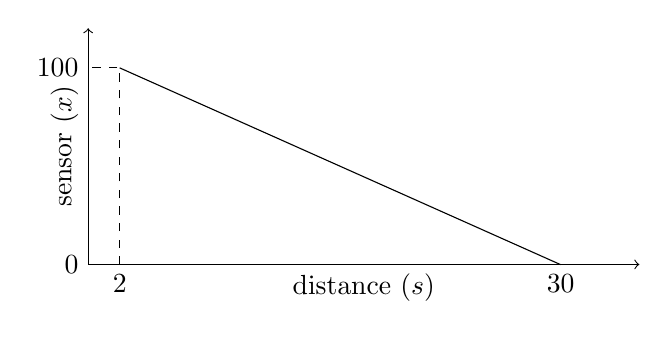
\begin{tikzpicture}
\draw[<->] (0,3) -- node[sloped,above,rotate=180] {\p{sensor ($x$)}} (0,0) node[left] {\p{0}} -- node[below] {\p{distance ($s$)}} (7,0);
\draw[dashed] (.4,0) node[below] {\p{2}} -- (.4,2.5) -- (0,2.5) node[left] {\p{100}};
\draw[domain=2:30] plot (\x/5,{(-3.57*\x+107)/40}) node[below] {\p{30}};
\end{tikzpicture}
\caption{Value returned as a linear function of distance}\label{fig.linear}
\end{center}
\end{figure}

Let us compute the slope and the intercept:
\[
\mathit{slope} = \frac{\Delta x}{\Delta s} = \frac{0-100}{30-2}=-3.57\,.
\]
When $s=30$, $x=0=-3.57\cdot 30+b$, so $b=107$ and $x = -3.57 s + 107$. Solving for $s$ gives a function that the robot's computer can use to map a sensor value to the corresponding distance:
\[
s = \frac{107-x}{3.57}\,.
\]

\begin{framed}
\act{Linearity}{linearity}
\begin{itemize}
\item Tape a ruler on your table and carefully place the robot so that its
front sensor is positioned next to the $0$ mark of the ruler. Place an object next to the $1$ cm mark on the ruler. Record the value returned by the sensor. Repeat for $2$ cm, $3$ cm, \ldots, until the value returned goes to zero.
\item Plot a graph of value returned vs. distance. Is the response of the sensor linear? If so, compute the slope and the intercept.
\item Repeat the experiment with objects of different shapes and materials. Does the linearity of the graph depend on the characteristics of the object?
\end{itemize}
\end{framed}

\subsection{Mapping nonlinear sensors}

Figure~\ref{fig.nonlinear} shows a possible result of the measurements in Activity~\ref{act.linearity}. The measurements are shown as dots together with the linear function from Fig.~\ref{fig.linear}. The function is reasonably linear in the middle of its range but nonlinear outside that range. This means that it impossible to use a linear function of the raw values of the sensor to obtain the distance of an object from the robot.

\begin{figure}
\begin{center}
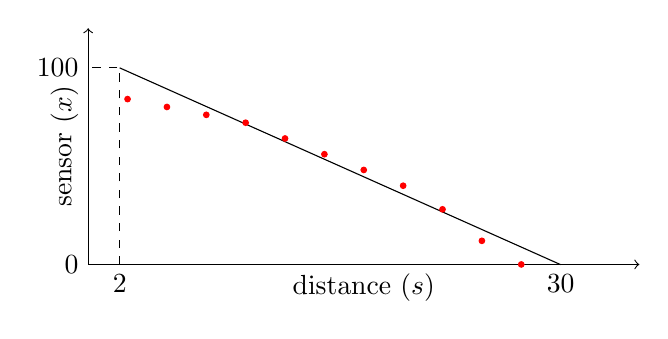
\begin{tikzpicture}
\draw[<->] (0,3) -- node[sloped,above,rotate=180] {\p{sensor ($x$)}} (0,0) node[left] {\p{0}} -- node[below] {\p{distance ($s$)}} (7,0);
\draw[dashed] (.4,0) node[below] {\p{2}} -- (.4,2.5) -- (0,2.5) node[left] {\p{100}};
\draw[domain=2:30] plot (\x/5,{(-3.57*\x+107)/40}) node[below] {\p{30}};
\foreach \x/\y in {0.5/2.5, 1/2.4, 1.5/2.3, 2/2.2, 2.5/2, 3/1.8, 3.5/1.6, 4/1.4, 4.5/1.1, 5/0.7, 5.5/0.4}
  \draw[fill,red,yshift=-4mm] (\x,\y) circle[radius=1pt];
\end{tikzpicture}
\caption{Experimental values returned as a function of distance}\label{fig.nonlinear}
\end{center}
\end{figure}

We can construct a table to map sensor values to distances. Table~\ref{tab.nonlinear} is a table based upon real measurements with an educational robot. Measurements were made every two centimeters from $2$ cm to $18$ cm; at $20$ cm the sensor no longer detected the object. The second column shows the value of the sensor for each distance. The third column shows the values $x_l$ that would be returned by the sensor if it were linear with the function $x=-2s+48$. We see that the actual values returned by the sensor do not deviate too much from linearity, so it would not be unreasonable to use a linear function.

\begin{table}
\begin{displaymath}
\begin{array}{r@{\hspace{2em}}r@{\hspace{2em}}r}
\svhline\noalign{\smallskip}
s \textrm{(cm)} & x & x_l\\
%\multicolumn{1}{c}{s \textrm{(cm)}} & \multicolumn{1}{c}{x}& \multicolumn{1}{c}{x_l}\\
\noalign{\smallskip}\svhline\noalign{\smallskip}
18 &14 & 12\\
16 &18 & 16\\
 14&22 & 20\\
 12&26 & 24\\
 10&29 & 28\\
 8 &32 & 32\\
 6 &36 & 36\\
 4 &41 & 40\\
 2 &44 & 44\\
\noalign{\smallskip}\svhline\noalign{\smallskip}
\end{array}
\end{displaymath}
\caption{A table mapping sensor values to distances}\label{tab.nonlinear}
\end{table}


Obviously, it would be better if we had a table entry for each of the possible values returned by the sensor. However, this would take a lot of memory and may be impractical if the range of values returned by the sensor is much larger, say, from $0$ to $4095$ ($12$ bits). One solution is to take the nearest value, so that if the value $27$ is returned by the sensor whose mapping is given in Table~\ref{tab.nonlinear}, the distance would be $12$.

A better solution is to use interpolation\index{interpolation}. If you look again at the graph in Fig.~\ref{fig.nonlinear}, you can see that the segments of the curve are roughly linear, although their slopes change according to the curve. Therefore, we can get a good approximation of the distance corresponding to a sensor value by taking the relative distance on a straight line between two points (Fig.~\ref{fig.interpolation}). Given distances $s_1$ and $s_2$ corresponding to sensor values $x_1$ and $x_2$, respectively, for a value $x_1<x<x_2$, its distance $s$:
\[
s = s_1 + \frac{s_2-s_1}{x_2-x_1}(x-x_1)\,.
\]

\begin{figure}
\begin{center}
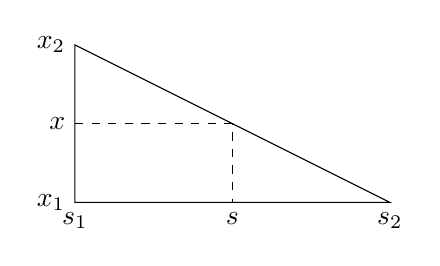
\begin{tikzpicture}
\draw (0,0) node[left] {$x_1$} -- (0,2) node[left] {$x_2$} -- (4,0) node[below] {$s_2$} -- cycle node[below] {$s_1$};
\draw[dashed] (0,1) node[left] {$x$} -| (2,1) -- (2,0) node[below] {$s$};
\end{tikzpicture}
\caption{Interpolation of sensor values}\label{fig.interpolation}
\end{center}
\end{figure}

\section{Summary}

When designing a robot, the choice of sensors is critical. The designer needs to decide \emph{what} needs to the measured: distance, attitude, velocity, etc. Then the designer has to make trade-offs: larger range, finer resolution, higher precision and accuracy are always better, but come at a price. For educational robots, price is the overriding consideration, so don't expect good performance from your robot. Nevertheless, the algorithmic principles are the same whether the sensors are of high quality or not, so the trade-off does not affect the ability to learn with the robot.

Any sensor connected to the robot's computer is going to return discrete values within a fixed range. The computer must be able to map these sensor values to physical quantities in a process called calibration. If the sensor is linear, the calibration results in two values (slope and intercept) that determine a linear function. If the sensor is nonlinear, a table or a non-linear function must be used.


\section{Further reading}

For an overview of sensors used in mobile robots see \cite[Section 4.1]{siegwart}. The book by Everett \cite{everett} is devoted entirely to this topic.

\bibliographystyle{spmpsci}
\bibliography{er}
